\chapter{编译、烧录与联机调试}
\label{ch:linkdebug}

\begin{introduction}
  \item 了解内置 SDCC C251 工具链：离线构建、指纹缓存与增量复用；
  \item 会读 \texttt{main.rst} 列表文件：地址、机器码、指令周期与 C 锚点；
  \item 会读 Intel HEX：记录结构、扩展地址与校验和；
  \item 理解 USB-HID 烧录协议：64 字节报告、128 字节 Flash 块与重发机制；
  \item 掌握烧录前后的供电开关、ISP 进入方式与失败排查。
\end{introduction}

第~\ref{ch:compileflash}~章用四步走通了“生成到固件进板子”。本章把每一步
拆开看：构建产物从哪里来、HEX 里写了什么、USB-HID 怎么把固件写进主控板、
失败了往哪里查。本章的代码与数据全部来自真实产物——用内置工具链编译
随书示例 \texttt{infantry-standard.pieproj} 得到 42092 字节的固件，
\texttt{debug-checklist.pieproj} 得到 36975 字节的固件。

\section{内置 SDCC C251：离线的完整构建}

“烧录”页的编译器有两个选项（图~\ref{fig:ch09-deploy}）：\textbf{内置
SDCC C251} 可完全离线使用；\textbf{Keil C251} 调用本机安装的 Keil。内置
SDCC 随应用发布，首次构建时把工具链与固件源码树部署到本地运行时目录，
之后按“指纹”复用：工具链清单、固件源码树内容与配置的哈希共同构成缓存
键，配置没变时再次构建直接命中缓存。

构建是一个多阶段流水线：把 \texttt{main.c} 与固件源码树的库文件逐个编译
成目标文件（示例配置共 22 个模块），再链接成 HEX，最后做布局与校验和
检查——\texttt{SDCC HEX/MAP 布局校验通过}之后，构建才算成功。构建日志
的每一步都会显示在“进度与日志”区。

\begin{figure}[htbp]
  \centering
  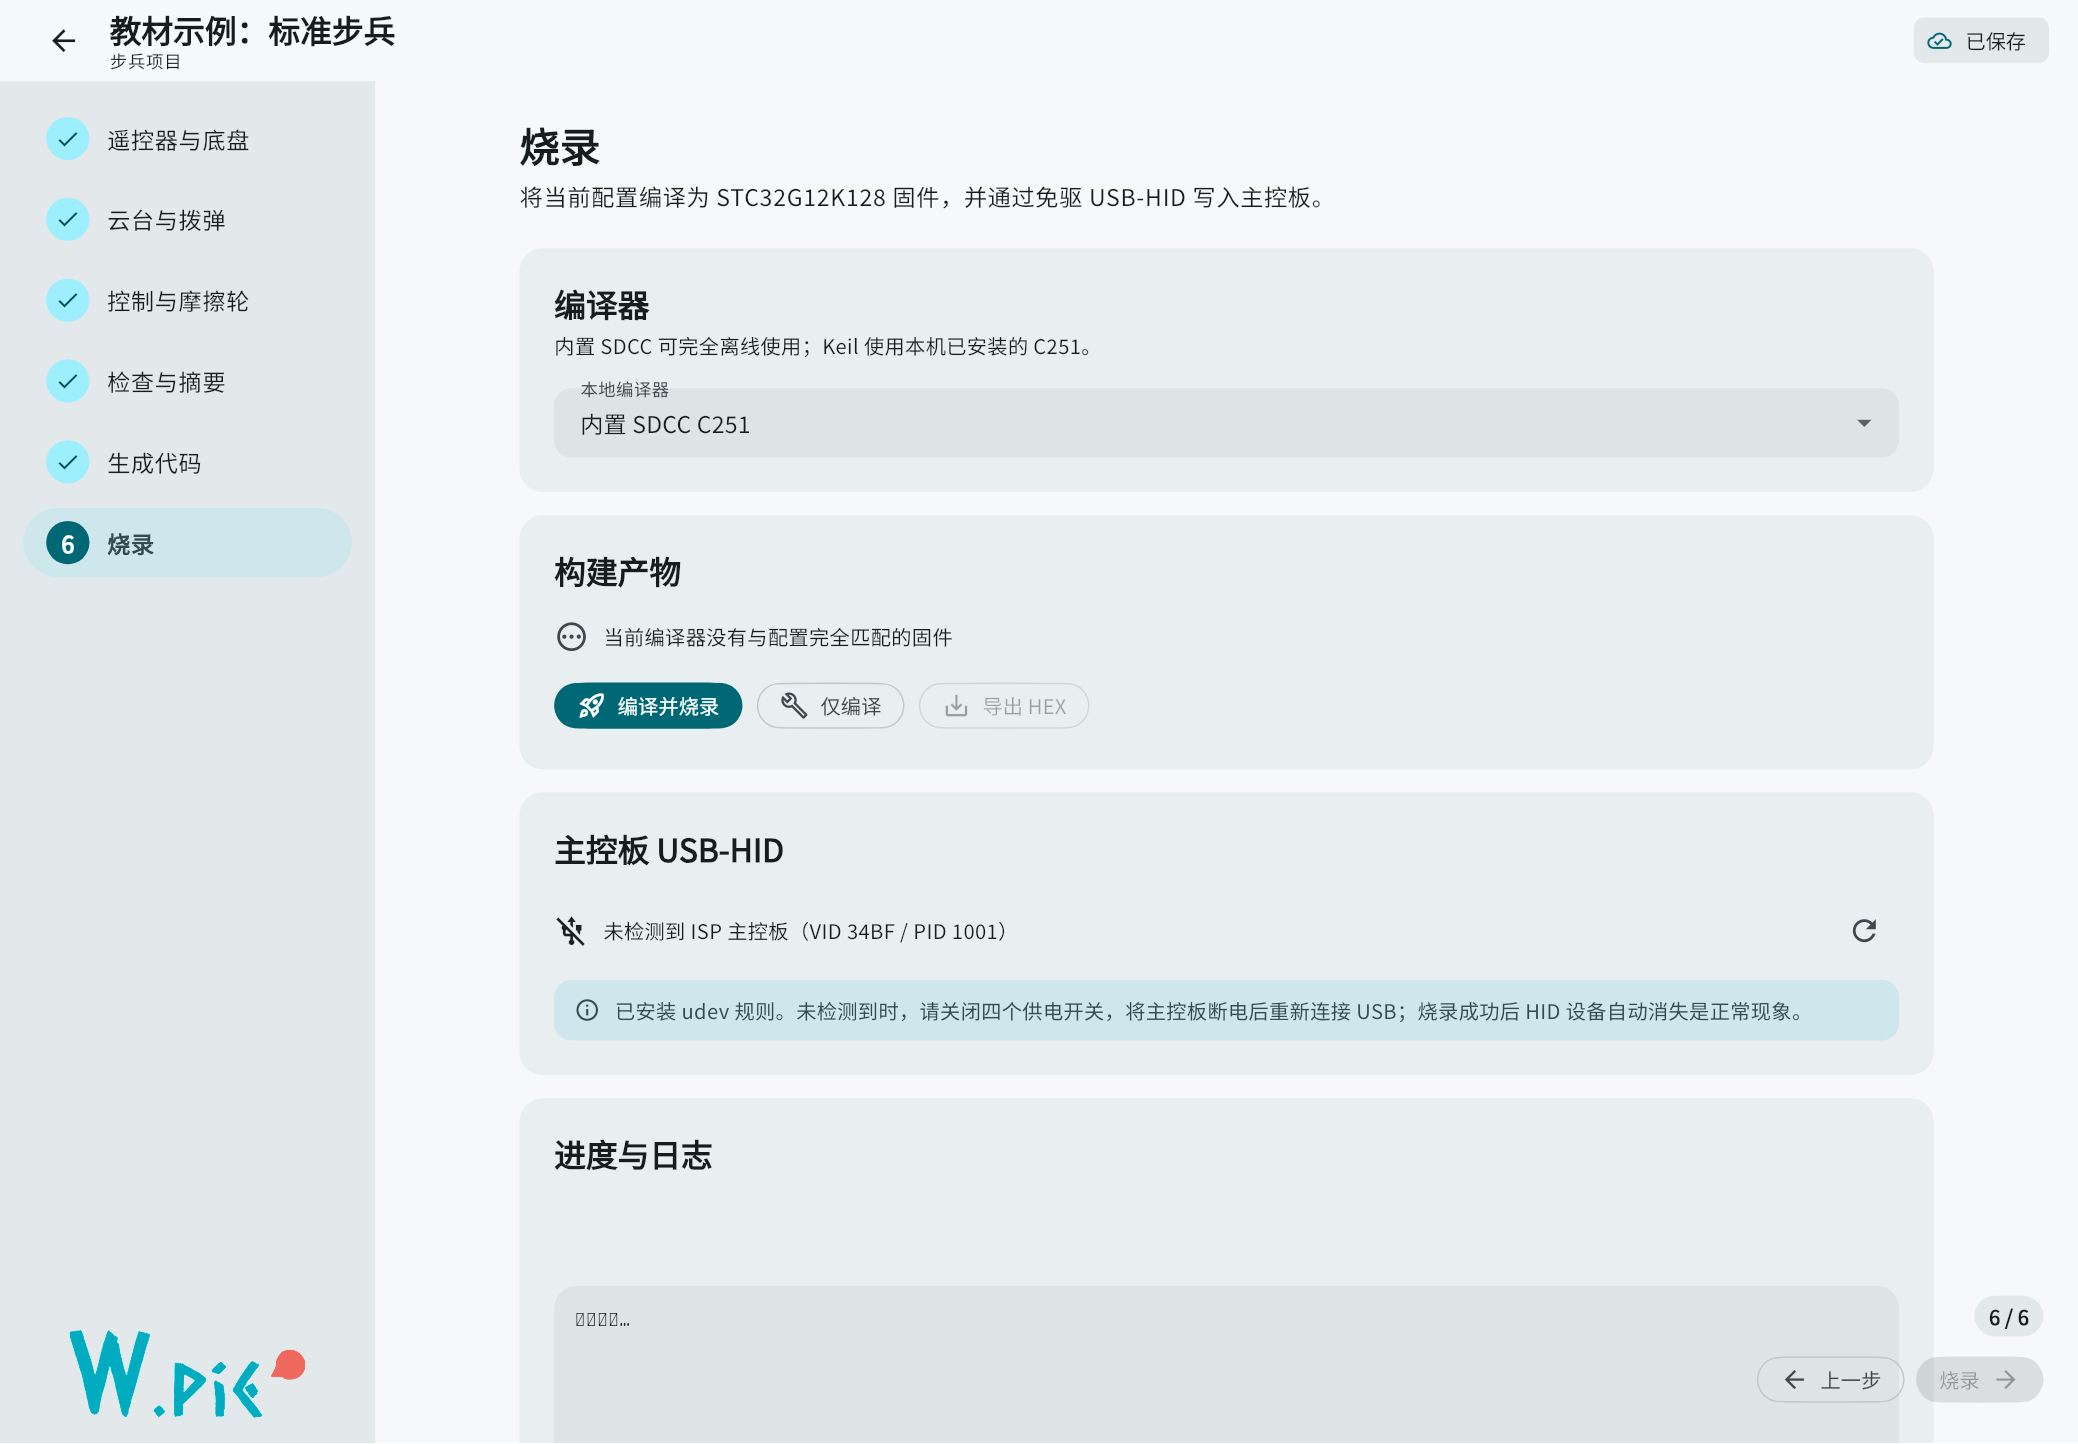
\includegraphics[width=0.95\linewidth]{image/ch09/9-1-deploy.png}
  \caption{“烧录”页：编译器选择、构建产物、主控板 USB-HID 检测与
  进度日志；未编译时“导出 HEX”不可用}
  \label{fig:ch09-deploy}
\end{figure}

Android 端使用随应用发布的 NDK 原生库（arm64-v8a / x86\_64）运行同一套
SDCC，通过 OTG USB-HID 烧录；Web 端没有本机工具链，编译与烧录都不可用，
但配置与生成代码照常工作（见第~\ref{ch:projects}~章）。

\section{列表文件 main.rst：C 与 251 指令的对照}

SDCC 构建完成后，“生成代码”页的“汇编”栏会显示链接后的列表文件
\texttt{main.rst}。它是研究 STC32G 编译结果的第一手材料：每一行给出
地址、机器码、指令周期与对应的 C 源码锚点。下面是调试固件里
\texttt{Ms\_Delay(duration)} 调用点附近的真实摘录：

\begin{lstlisting}[style=pieblockc,
  caption={\texttt{main.rst} 真实摘录：地址、机器码、周期、汇编与 C 锚点},
  label={lst:ch09-rst}]
      FE05A0 D0 06            [24] 1135 	pop	ar6
      FE05A2 D0 07            [24] 1136 	pop	ar7
                                   1137 ;	.../main.c:67: Ms_Delay(duration);
      FE05A4 69 1F FF FC      [12] 1138 	mov	wr2,@spx-0x0004
      FE05A8 7A 31 82         [12] 1139 	mov	dpl, r3
      FE05AB 7A 21 83         [12] 1140 	mov	dph, r2
      FE05AE C0 07            [24] 1141 	push	ar7
      FE05B0 C0 06            [24] 1142 	push	ar6
      FE05B2 C0 05            [24] 1143 	push	ar5
      FE05B4 C0 04            [24] 1144 	push	ar4
      FE05B6 9A FE 02 F4      [12] 1145 	ecall	_Ms_Delay
      FE05BA D0 04            [24] 1146 	pop	ar4
\end{lstlisting}

方括号里是 251 内核的指令周期数。一行 C 展开成几条指令、参数怎样装进
寄存器（\texttt{dpl/dph} 是参数的低/高字节）、调用如何传栈帧，都能在
这里逐条对上。研究汇编可以回答“这个表达式实际编译成了什么”，是
第~\ref{ch:engineer}~章里“int 乘法不提升到 32 位”一类论断的验证工具。

\section{Intel HEX：固件的文本形态}

“导出 HEX”把构建产物存成 Intel HEX 文件——一种文本格式的固件镜像。
每行一条记录：

\begin{lstlisting}[style=pieblockc,
  caption={随书步兵固件 HEX 的首、尾记录（真实数据）},
  label={lst:ch09-hex}]
:0200000400FEFC
:2000B400E49000037584017AEBB074809000027584017AEBB074519000017584017AEBB0AC
:2000D40074019000007584017AEBB043BA8090FE0175847E7F7E74047AEBB090FDEB75847A
...
:17A3B80095F040048AFEA3C77582018AFEA3CA7582001BFE1BFEAA13
:00000001FF
\end{lstlisting}

每行以冒号开头，依次是：本行数据字节数、16 位地址、记录类型、数据、
单字节校验和（本行所有字节之和取负）。记录类型 \texttt{04} 是扩展线性
地址：第一行 \texttt{:0200000400FEFC} 表示“后续数据的高 16 位地址是
\texttt{0x00FE}”，即固件主代码位于 \texttt{0xFE0000} 起的映射区；
\texttt{00} 是数据记录（\texttt{:20} 即 32 字节一行）；最后一行
\texttt{:00000001FF} 是文件结束。烧录器会把记录重新拼装成按地址索引的
字节镜像，并逐字节核对校验和——所以 HEX 文件被手改一个字符都会在校验
时暴露。

\section{USB-HID 烧录协议}

主控板的 STC32G 出厂引导程序（ISP）以 USB-HID 设备的身份出现，VID
\texttt{34BF}、PID \texttt{1001}——页面“主控板 USB-HID”卡片检测到的
就是它。HID 是免驱协议：操作系统不需要驱动，应用直接用 64 字节的报告
（report）与设备交换数据。

烧录协议的要点：

\begin{itemize}
  \item \textbf{包结构}：每条命令封成一个包——帧头 \texttt{46 B9 6A}、
        两字节总长、载荷、两字节累加和、帧尾 \texttt{16}；超过 64 字节
        的包按 64 字节报告分片发送；
  \item \textbf{按块写入}：HEX 镜像按 128 字节一块对齐，逐块下发。第一块
        用命令 \texttt{0x32}，后续块用 \texttt{0x12}；地址超出低 64KB
        应用区的部分映射到高区（\texttt{0xFF0000} 起），用命令
        \texttt{0x02}；
  \item \textbf{应答与重发}：每块写完等设备应答；无响应时自动重发若干次
        并在日志里提示“无响应，正在重发”，连续失败才中止烧录。日志区
        会显示块地址与进度。
\end{itemize}

\begin{note}
\textbf{只能烧主控板，绝不能向机械拓展板烧录程序}——拓展板的固件由学长
学姐预先烧好，被误擦除需要付费恢复。烧录前应关闭四个供电开关：主控板的
SERVO、POWER 与拓展板的 POWER、BOOSTER，避免无法识别或电流倒灌；已关闭
时按“已关闭开关，继续烧录”确认即可。
\end{note}

主控板必须通过断电重新上电进入 ISP 模式：已运行固件的芯片不会一直停留在
HID 模式，所以“烧录成功后 HID 设备自动消失是正常现象”；再次烧录前要
重新断电上电。Linux 下首次烧录需要安装 udev 规则（应用会弹出系统授权
对话框，把 hidraw 授权规则写入 \texttt{/etc/udev/rules.d/70-pieblock-
hid.rules} 并重载）；规则装好后若仍检测不到，请拔插或断电重新上电。

\section{Keil C251 与失败排查}

选择 Keil 编译器时，需要告诉 PIE-Block 本机 Keil 的安装目录（也可以用
环境变量指定）。应用会把 C251 许可证密钥写入 Keil 的
\texttt{TOOLS.INI}——写入前会先备份该文件，密钥本身不保存在 PIE-Block
的任何位置。Keil 构建的入口是 \texttt{uVision.com} 命令行（不是 GUI 的
\texttt{UV4.exe}）；\textbf{退出码不可靠}——编译完全成功时它也可能返回
非零，唯一可靠的判据是日志里出现 \texttt{0 Error(s)}。

烧录与编译的常见失败见表~\ref{tab:ch09-trouble}，更多高频问题见
附录~B。

\begin{table}[htbp]
  \centering
  \small
  \begin{tabularx}{\linewidth}{@{}>{\raggedright\arraybackslash}p{0.30\linewidth} >{\raggedright\arraybackslash}X@{}}
    \toprule
    现象 & 处理 \\
    \midrule
    未检测到 ISP 主控板 & 关闭四个供电开关，主控板断电重新上电进 ISP；Linux 先装 udev 规则并重新插拔 \\
    写块无响应 & 多为供电或线缆问题：换 USB 口/线，关闭供电开关重试；应用会自动重发若干次 \\
    首次部署 SDCC 失败 & 常见于中文用户名路径或杀毒软件占用运行时目录，按页面提示处理（详见附录~B） \\
    Keil 找不到 C251.EXE & 检查 Keil 目录选择与 \texttt{TOOLS.INI} 的 \texttt{[C251]} 段路径；必要时重新应用许可证 \\
    编译“失败”但日志 0 Error & Keil 退出码不可信：以日志 \texttt{0 Error(s)} 为准 \\
    烧录成功但设备消失 & 正常现象：固件启动后退出 ISP；重新烧录需断电重上电 \\
    \bottomrule
  \end{tabularx}
  \caption{编译与烧录类问题速查}
  \label{tab:ch09-trouble}
\end{table}

烧录成功只是开始。接下来的“联机调试”在实车上按
第~\ref{ch:debugproj}~章的检查单逐项验证，把配置、代码与硬件之间最后的
偏差找出来——固件进板子只是把“纸面正确”变成了“可验证”，验证本身
仍然要人来做。
